\documentclass[10pt,a4paper]{report}
\usepackage[utf8x]{inputenc}
\usepackage{ucs}
\usepackage{amsmath}
\usepackage{amsfonts}
\usepackage{amssymb}
\usepackage{graphicx}
\usepackage{Sweave}
\author{Dorottya Cserpan}

\begin{document}

\section{kCSD for Ballstick Modell}




Parameters:

\begin{Schunk}
\begin{Soutput}
Number of electrodes: 10
\end{Soutput}
\begin{Soutput}
Number of base functions: 18
\end{Soutput}
\begin{Soutput}
Type of base functions: step
\end{Soutput}
\begin{Soutput}
Width of base functions: 30 um
\end{Soutput}
\begin{Soutput}
sigma: 0.5
\end{Soutput}
\begin{Soutput}
Shift of overlapping of base functions: 27.7777777777778 um
\end{Soutput}
\begin{Soutput}
Cell to electrode distance: 30
\end{Soutput}
\end{Schunk}

Units:
\begin{Schunk}
\begin{Soutput}
Potential 	  [mV]
\end{Soutput}
\begin{Soutput}
Current      [nA]
\end{Soutput}
\begin{Soutput}
Conductivity [S/m]
\end{Soutput}
\begin{Soutput}
Dimension 	  [μm]
\end{Soutput}
\end{Schunk}




\begin{Schunk}
\begin{Soutput}
X11cairo 
       2 
\end{Soutput}
\end{Schunk}
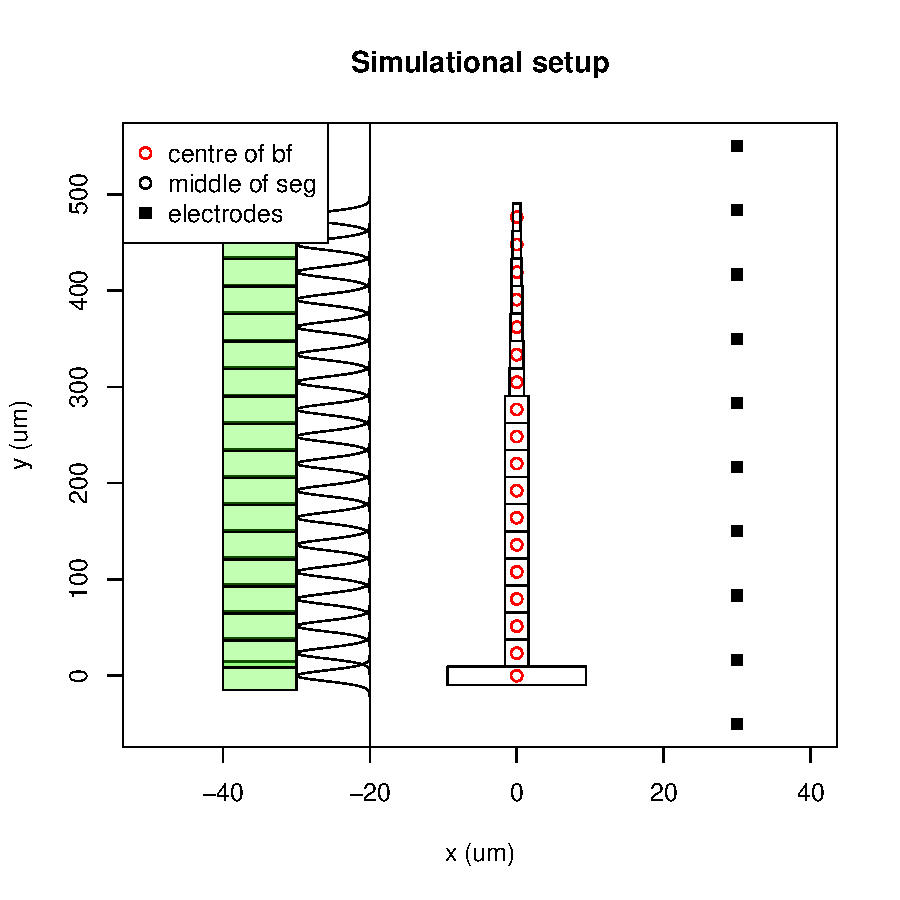
\includegraphics{bs_1D_130506-setup}

\includegraphics{bs_1D_130506-elefpes}



Nem vagyok benne biztos, hogy ez jó...
Most kell kiszámolni az adott pontforrásokban a különböző Gaussok amplitúdóját és azokat összeadni, ezt egy mátrixban a legegyszerűbb ábrázolni. A sorok a különböző pontforrásokat jelzik, az oszlopok a különböző Gauss függvényeket, a rácspontokban az amplitúdók állnak...
\includegraphics{bs_1D_130506-Cstar}

\includegraphics{bs_1D_130506-membcurrentplot}

\includegraphics{bs_1D_130506-imagemebc}



\includegraphics{bs_1D_130506-tobbiresz}



\begin{Schunk}
\begin{Soutput}
Overall RMSE 0.0110068825671664
\end{Soutput}
\end{Schunk}
\includegraphics{bs_1D_130506-014}

\includegraphics{bs_1D_130506-CSD}


Spatial distribution at spike:
\includegraphics{bs_1D_130506-spatialspike}

\includegraphics{bs_1D_130506-spatialspike2}
\begin{Schunk}
\begin{Soutput}
Spike rmse: 0.0517455859301027
\end{Soutput}
\end{Schunk}
\end{document}

